\begin{minipage}[c]{0.5\textwidth}
    [m3102719e]\quad
    如图所示,图中是某中学初一(1)班某次期中考试成绩各个分数段人数的统计图
    已知其中不及格同学的人数占全班人数的$\dfrac{1}{13}$。 \par
    (1) 初一(1)班共有多少学生? \par
    (2) 成绩在80-90分的同学人数全班人数的人数几分之几? \par
    (3) 成绩60-70分的人数比80-90分的同学人数少几分之几?
\end{minipage}
\begin{minipage}[c]{0.5\textwidth}
    \begin{figure}[H]
        \centering
        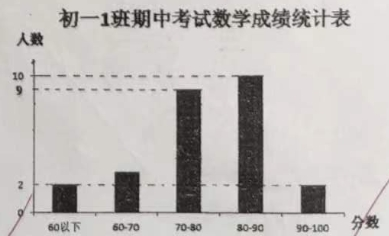
\includegraphics[width=0.9\textwidth,keepaspectratio]{m3102719eb}
    \end{figure}
\end{minipage}   
\AnswerBox{m3102719ea}{0.9}{20}